\documentclass[../main.tex]{subfiles}
\begin{document}
    \begin{center}
        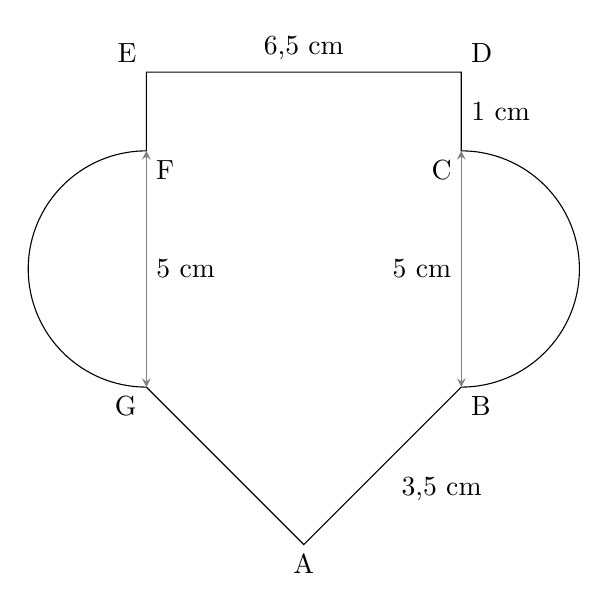
\begin{tikzpicture}
            \coordinate[label=below:A](A)at(0,-1);
            \coordinate[label=below right:B](B)at(2,1);
            \coordinate[label=below left:C](C)at(2,4);
            \coordinate[label=above right:D](D)at(2,5);
            \coordinate[label=above left:E](E)at(-2,5);
            \coordinate[label=below right:F](F)at(-2,4);
            \coordinate[label=below left:G](G)at(-2,1);
            \draw(A)--(B)arc(-90:90:1.5)--(D)-%
            -(E)--(F)arc(90:270:1.5)--cycle;
            \tkzMarkSegment[color=vscode-crimson,mark=s||](A,B)
            \tkzMarkSegment[color=vscode-crimson,mark=s||](G,A)
            \tkzMarkSegment[color=vscode-crimson,mark=s|](E,F)
            \tkzMarkSegment[color=vscode-crimson,mark=s|](C,D)
            \draw[stealth-stealth,line width=0.4 pt, color=gray](G)--(F)
                node[pos=0.5,shift={(0.5,0)},color=black]{5 cm};
            \draw[stealth-stealth,line width=0.4 pt, color=gray](C)--(B)
                node[pos=0.5,shift={(-0.5,0)},color=black]{5 cm};
            \path(A)--(B)node[pos=0.5,shift={(0.75,-0.3)}]{3,5 cm};
            \path(D)--(C)node[pos=0.5,shift={(0.5,0)}]{1 cm};
            \path(E)--(D)node[pos=0.5,shift={(0,0.3)},color=black]{6,5 cm};
        \end{tikzpicture}
    \end{center}
    \begin{enumerate}[1),font=\bfseries]
        \item Décrire la figure ci-dessus en utilisant le vocabulaire adapté
        (cercles, segment,...).
        \ncar5\dotedline
        \item Calculer le périmètre de la figure ci-dessus.
    \end{enumerate}
\end{document}